\hypertarget{cct}{%
\chapter{City of Cape Town, South Africa: Aligning Internal Data Capabilities with External Research Partnerships}\label{cct}}

\printchapterauthor{%
\begin{authorlist}
  Hugh Cole (City of Cape Town)  \\
  Kelsey Jack (University of California, Santa Barbara)  \\
  Derek Strong (University of Southern California)  \\
  Brendan Maughan-Brown (University of Cape Town)  \\
\end{authorlist}}\authorfootnote{Cole, Hugh, Kelsey Jack, Derek Strong, and Brendan Maughan-Brown}{Hugh Cole, Kelsey Jack, Derek Strong, and Brendan Maughan-Brown}{cct}
\authortoc{Hugh Cole, Kelsey Jack, Derek Strong, Brendan Maughan-Brown}
\hrulefill

\hypertarget{summary-6}{%
\section{Summary}\label{summary-6}}

The day-to-day administration of policies and programs in the City of Cape Town (CCT), South Africa generates a large amount of data. In recent years, decision-makers in CCT have begun to think strategically about how to leverage these data resources to tackle multiple and interrelated municipal policy challenges, including the sustainability of utility services (e.g., energy and water); rapid urban transformation; investments in transportation, housing, and infrastructure; the informal economy; and public safety. Specifically, CCT has made initial investments in enhancing data capabilities by adopting and implementing a data strategy and establishing a Data Science unit to facilitate greater data sharing (including through data engineering), enhanced tools for analysis (including open-source tools and data science environments), and advanced analytics. This builds on many years of investment in research, data, statistical analysis, and corporate (as opposed to fragmented) GIS capability. It also builds on the development of sophisticated policy and strategy capacity and a single policy development process for the whole organization. These steps have laid the groundwork for a broad-based effort to adopt evidence-based policymaking for greater impact and more cost-effective solutions.

Evidence-based policymaking is built on research informed by policy-relevant data sets. Practically, this requires making data available to researchers both within the municipal government and outside of it, primarily but not exclusively in academia. Data access presents numerous new challenges associated with the scale and scope of administrative data and the human resource and technological capabilities to use and share data. Specific concerns, common to many administrative contexts but particularly challenging at the municipal level, include (i) the security challenges of data sharing, (ii) the legal risks associated with greater data access, and (iii) the time and resource investment required to maintain the data architecture and governance systems that enable the sharing and use of data by various actors.

CCT maintains active research collaborations with numerous partners, which have helped to identify policy and program strengths and areas for improvement. This chapter emerges out of such a collaboration, between CCT and researchers at the Abdul Latif Jameel Poverty Action Lab (J-PAL) and University of California, Santa Barbara (UCSB), and reflects contributions from both sides of the research-policy interface. The authors describe ongoing efforts to develop a more streamlined system for cataloging, accessing, and sharing administrative data with external researchers and with analysts and decision-makers within CCT. The partnership has worked together over the past two years to advance CCT's vision for streamlined data sharing. Bringing researchers into the planning and implementation process helps to ensure that data sharing solutions work for both policy and research. The end goal is a single, cloud-based, data sharing platform for both public-use and restricted-use data sets, documented in a browsable catalog with standardized metadata. The single platform would be used by researchers both inside and outside of the city government. A streamlined process for research permission and data access would increase researcher accountability, including the reciprocal sharing of research output, analysis code, and cleaned and new data sets. The work is still in progress and the descriptions in this chapter reflect the evolving situation.

\hypertarget{introduction-7}{%
\section{Introduction}\label{introduction-7}}

\hypertarget{motivation-and-background-5}{%
\subsection{Motivation and Background}\label{motivation-and-background-5}}

Municipalities in South Africa play numerous roles: first, providing democratic and accountable government for local communities; second, ensuring service provision to communities in a sustainable manner; third, promoting social and economic development; fourth, encouraging the involvement of communities and community organizations in the matters of local government. The City of Cape Town is no exception. It serves a population of over 4 million people and provides a mix of basic services (electricity, water, sanitation, and refuse removal) and supporting services (transport, housing, safety, emergency services, primary healthcare, environmental health, community development, environmental services, and digital infrastructure) with a \href{http://resource.capetown.gov.za/documentcentre/Documents/Financial\%20documents/1920AdjBudget_Ann1_1_OpexAdjSummary_May2020.pdf}{2020 operating budget} of around US\$3 billion. Relative to many municipalities around the world, CCT's data systems are well organized and well maintained. For example, all formal commercial and residential properties are registered on cadastral maps and assigned a unique parcel number to which other municipal records, including property taxes, water, electricity and refuse billing, and other services are linked. This has facilitated administrative innovations, such as \emph{consolidated billing}: many businesses and residents receive a single bill for their municipal account, which streamlines the process of collections and accounting. However, these data remain under-utilized for purposes other than administration and operations. Specifically, while capacity for data analytics and research within CCT continues to grow, even internal staff struggle to identify, obtain, and process the necessary data.

Recent crises, including the 2017--18 water crisis (``Day Zero'') and the 2020 COVID-19 pandemic, highlight the importance of internal data sharing and analytics. They also revealed challenges. For example, staff in one department may be unaware of the data collected by another department, unsure of how to link data sets across departments, and unfamiliar with the staff members who manage the other data. Parallel challenges arise around research partnerships with external actors whose specific and often one-off data requests impose a time burden on CCT staff; these actors often lack engagement both in developing research questions and sharing results. Historically, the data sharing process for external parties has proceeded on a case-by-case basis. This ad hoc approach is costly for both data providers and researchers, and it often depends on personal relationships. These relationships may unravel if CCT staff change jobs and result in opportunistic collaborations that may miss some of the most high-value opportunities. Additionally, the actual transfer of data is not always secure (e.g., sometimes involving unencrypted flash drives). In spite of these challenges, CCT has engaged in successful research collaborations with external partners on topics including water conservation, municipal tariffs, electricity metering, youth employment, and more.

The situation has started to change. In 2016, Cape Town's municipal government underwent a restructuring process. As part of that process, CCT leaders looked to other cities around the world to collect innovative ideas for how to better run a fast-growing urban hub in a middle-income country. A theme emerged: leveraging the data created as part of regular administration and operation had the potential to uncover opportunities and efficiencies, leading to more effective governance and policymaking. The restructuring created two new units that are central to the activities described in this chapter: (1) a Policy and Strategy Department and (2) a Data Science unit. Craig Kesson, now executive director of Corporate Services at CCT, was a champion and architect of steps to strengthen evidence-led decision-making and data capabilities. Hugh Cole (one of the authors on this chapter) was recruited from the International Growth Centre (IGC) at the London School of Economics to lead the Policy and Strategy Department. While at the IGC, Hugh saw first-hand the potential for evidence to inform and improve policy and the crucial role that administrative data play in opening up collaborations between policymakers and researchers. Within the CCT, he began to advance an agenda for streamlining research collaborations, building internal research capacity, and making data more accessible to researchers both inside and outside of the CCT government.

In parallel, Kelsey Jack (another author on this chapter) had developed a series of collaborative research activities with CCT and researchers at the University of Cape Town where J-PAL's Africa regional office is based. As described in greater detail in the Data Use Examples, these collaborations revealed both the strengths of CCT's administrative data and areas for improvement. Kelsey and Hugh were in regular contact about the challenges of identifying, accessing, and working with CCT data sets. In 2018, Kelsey hired Derek Strong (a third author on this chapter) to work with both the Policy and Strategy and Data Science units within CCT to identify and advance solutions to these challenges. Importantly, the barriers faced by external researchers, both internationally and in Cape Town, were paralleled by researchers and data analysts within the municipal government. Thus, any progress toward data organization and access would be of immediate value to both internal and external actors.

While efforts to streamline data access in CCT are ongoing, including the expansion of remote access to data, substantial time and resources have already been invested under the CCT, J-PAL, and UCSB collaboration. From the researchers' perspective, the motivation appears clear: access to high-quality administrative data from a globally important city presents exciting opportunities. Furthermore, remote access to data also enables more convenient, international collaborations and even removes the need for a physical presence in Cape Town.

CCT's motivation to devote time and resources to such an endeavor stems both from a desire to uncover creative solutions to combat persistent, urban challenges and to establish terms for research partnerships that are more collaborative, building internal capacity and filling data gaps. As an example of the former, the investment of time and expertise by external researchers can uncover new policy insights that go beyond the scope of internal data analytics. Similarly, more accessible and user-friendly data resources lower the cost of incorporating data and evidence into the internal decision-making process. As an example of the latter, high levels of informality in the housing, transport, and economic sectors lead to persistent gaps in administrative records. Research collaborations involving primary data collection and analysis relevant to the informal sector complement administrative data and help inform a more relevant and responsive regulatory and service delivery environment for the most vulnerable residents. However, streamlined data sharing and reciprocal agreements are needed to achieve this collaborative vision.

The desire to fully capture the value of data and to streamline data sharing led CCT to adopt and implement a \emph{Data Strategy} in June 2018.\footnote{A summary of implementation activities associated with the Data Strategy is provided at \url{http://osf.io/2a7ev}. The document is not yet publicly available but will be provided at this same location when it becomes available.} This strategy recognizes administrative data as a ``collection of public assets that should be managed in a way to maximize public benefit and organizational growth.'' It describes how CCT intends to transform its data for greater utilization and the management and processes surrounding CCT data to support meaningful strategic and operational decision-making. As part of the Data Strategy, CCT is currently developing more streamlined data management processes along with tools to lower the cost of sharing and coordinating across data sets both internally and externally. The Data Strategy resulted in the creation of the new role of chief data officer, which is a role fulfilled by Craig Kesson (in addition to his executive director functions).

A \emph{Research Framework} adopted in 2019, also clarifies procedures for sharing data with external partners by integrating data access into broader research management practices to ensure reciprocal exchange of value and the translation of knowledge into policy.\footnote{The City's Research Framework outlines a collection of systematic approaches to help the effective and efficient production, flow, and use of information and knowledge in the organization. The framework comprises a research vision, research value chain, and enablers (research principles, objectives, and activities), and includes a high-level CCT Research Agenda that outlines the City's priority research themes. The document is not yet publicly available.} As described in the Research Framework, research needs are evaluated in the development or revision of all CCT policies, strategies, and bylaws. The identified research needs are then incorporated into CCT's \emph{Research Agenda} to inform what research CCT procures or pursues in the form of partnerships.

By aligning internal data capabilities with external research partnerships, the Data Strategy and Research Framework facilitate collaborative research. Primary issues raised in these documents include data accessibility (lack of documentation and mechanisms to identify and obtain data), data quality (multiple versions of related transactions), data custodianship (uncertain or ambiguous accountability), data security (lack of consistent guidelines and practices), and data analytics (lack of capabilities).

\hypertarget{data-use-examples-5}{%
\subsection{Data Use Examples}\label{data-use-examples-5}}

This section discusses three data use examples that have been catalytic for the collaboration underpinning this chapter and occurred prior to the streamlining efforts described, then introduces a third case that highlights ongoing challenges. The first data use example describes in detail the challenges and opportunities around making data available to external research partners. The other two exemplify the importance of data for internal analytics and decision-making and raise many of the same lessons described under the external data use example. These examples are intended to provide grounding for the challenges and potential solutions discussed in the rest of the chapter.

\hypertarget{case-1-impacts-of-pre-paid-electricity-metering}{%
\subsubsection*{Case 1: Impacts of Pre-Paid Electricity Metering}\label{case-1-impacts-of-pre-paid-electricity-metering}}
\addcontentsline{toc}{subsubsection}{Case 1: Impacts of Pre-Paid Electricity Metering}

Like many research partnerships, this first example arose out of an existing research relationship. As part of his master's thesis at the University of Cape Town (UCT), Grant Smith had collaborated with Professor Martine Visser on a project involving water billing data \citep{smith2014} and expanded his research to include analysis of both water and electricity data as part of his PhD dissertation. To facilitate this work, Grant Smith (through UCT) established a data use agreement\index{data use agreement} (DUA) with the water and electricity departments of CCT that allowed for broad access to utilities data. Kelsey Jack was added to this existing DUA through an addendum process once she and Grant began collaborating. The research project arose out of an initial interest in understanding how prepayment for electricity affected residential customers. Prepaid metering of electricity is common across Africa but little research had been done to understand how it impacts customers or electric utilities. A series of meetings between the researchers and staff in CCT's electricity department revealed an opportunity for a randomized controlled trial to measure the impacts of prepaid electricity metering relative to monthly billing. The experiment utilized an existing program, which replaced several postpaid or conventional meters with prepaid meters, by randomizing the order of meter replacement. The origin story of this case highlights the role of personal relationships and familiarity with available data, along with the value of genuine collaboration to identify questions and opportunities for research partnerships.

The project required data provisions by three distinct parties. First, billing data were accessed through the Systems Applications and Products in Data Processing (SAP) server (used to manage household bills) under the Enterprise Resource Planning department. Second, prepaid electricity data were accessed from the server used to administer the point of sale vending system under the Electricity department. Finally, GIS data necessary to support the spatial randomization design were accessed through the GIS team in the Electricity department. In parallel, researchers worked closely with operational staff unfamiliar with the details of data management, access, and processing. Researchers therefore iterated between data extraction requests (typically done in-person with the relevant data manager and involving file downloads on to CDs or flash drives) data cleaning, and design decisions. This process highlighted the value of centralized data inventories and a streamlined process for data sharing to lessen the time burden on both sides.

Once data were obtained from CCT, the process of integrating the data with the logistics of a field experiment was extremely time consuming. The RCT involved around 4,000 customers, but the data sets covered all residential electricity customers in CCT. These were used as inputs to the randomization to ensure balance on observable characteristics such as electricity use and property values. In addition, researchers worked with the operational staff to ensure adherence to the randomization and to match implementation details with the administrative outcome data on the back end. In practice, this involved daily visits to the office of the contractor hired to implement the meter replacements to reconcile their records with those of the research team.

Administrative records were used not just as an input to the randomization but also as the primary source of outcome data. This required numerous steps to ready the data for analysis. First, the most complete format for accessing billing records involves text files associated with printing a household's bill. Bill formats change periodically, and bills can be printed in three different languages. Extracting the relevant information from these files required extensive processing. Second, once households were switched from electricity billing to prepaid metering, the system used to track their electricity use changed from the SAP-based billing records to the prepaid point-of-sale vending records. Linking these two systems relied on property identifiers. Third, in lieu of shareable metadata to explain the data sets, the principal investigators (PIs) and research assistants relied on extensive direct communication with data managers, including in-person meetings, e-mails, and telephone calls. In many cases, these conversations were prompted when efforts to clean or organize data hit roadblocks. As a result, the cleaning process was less efficient and the communication less streamlined than if more complete metadata had been available at the start. Similar requests are likely fielded from other researchers working on the same or related data, forcing CCT staff to repeat information.

Given the nature of the study design, data could not be completely de-identified. In particular, it was necessary to retain both meter numbers (for prepaid and postpaid data sets) and property identifiers, which were used to match across data sets and implement the spatial randomization. However, all other identifiers (names, addresses, etc.) were removed in an initial step of cleaning done at UCT on a secure server. In some cases, requests were made at the time of data extraction to only share the necessary identifiers. However, it was often easier for the CCT data manager to impose minimal filters on the data at the time of extraction rather than customizing the fields for each request, and it was left to the UCT-based research team to complete the de-identification process prior to cleaning and analysis. As a result, the information loaded onto flash drives and CDs often contained detailed information, including names and addresses.

Upon completion of the project, the PIs solicited feedback from CCT on the research findings through (1) a presentation to the Electricity department, (2) a presentation to the head of the utilities division, and (3) sharing the draft manuscript with a request for comments. The DUA required CCT be given thirty days to review the manuscript for disclosure of confidential information. No specific comments were directed toward confidentiality or disclosure control. Efforts on the part of the researchers to solicit feedback above and beyond the required confidentiality review were voluntary and organized by the researchers.

The paper was published in a journal that requires non-confidential data be published alongside the manuscript \citep{jack2020}. The PIs provided code, detailed metadata, and instructions for how to request the data for replication directly from CCT. However, providing instructions with sufficient detail for actual replication was near-impossible. Standardized data sets shared through a streamlined data sharing platform would facilitate replication: code could be published along with instructions referencing specific data sets and variables.

\hypertarget{case-2-data-use-for-planning-and-policy-during-cape-towns-drought}{%
\subsubsection*{Case 2: Data Use for Planning and Policy During Cape Town's Drought}\label{case-2-data-use-for-planning-and-policy-during-cape-towns-drought}}
\addcontentsline{toc}{subsubsection}{Case 2: Data Use for Planning and Policy During Cape Town's Drought}

The recent drought in Cape Town (2015--18) required CCT to engage with both external researchers and with its own data in new ways to support decision-making in a time of crisis. In this case, a crucial step involved sharing and visualizing data on water supply and consumption to keep Cape Town's population informed and spur collective action to conserve water. Specifically, CCT made use of data visualization to keep citizens informed by developing a \href{https://coct.co/water-dashboard}{\emph{Water Dashboard}} that reflected dam storage percentages, weekly dam level changes, and average daily production. Additionally, a city water map known as the Green Dot map depicted household water consumption levels across specified bands of kiloliter usage.\footnote{Though the map has been removed from CCT's website, information on the map is available at \url{http://www.capetown.gov.za/Family\%20and\%20home/Residential-utility-services/Residential-water-and-sanitation-services/cape-town-water-map}} This provided a neighborhood lens on water usage and allowed for targeted communication and peer influencing to motivate behavior change (reducing household water consumption).

Furthermore, by harnessing and monitoring detailed, high-frequency data, the City was able to increase the efficiency of existing water infrastructure. For example, pressure reducing valves (PRVs) were used to provide data on pressure and flow in order to inform and optimize the operation of the water infrastructure. Through the use of PRVs, demand and leakage within a distribution system was managed more efficiently by reducing pressure in a discrete zone. The installation of PRVs provided valuable data that helped to improve reliability of service delivery, decrease infrastructure damage and water losses, and forecast and budget for repairs. Subsequent advanced analytics using PRV data were, however, limited by the data provisions in the PRV supplier contracts; CCT will seek to avoid this in future contracts.

The drought highlighted the complexity and importance of spatially explicit, real-time data access, the value of visualization, and the issues with combining different data sources. Data sharing was crucial to CCT's success in reducing water consumption to a level that allowed CCT to make it through the drought. The drought also illuminated data challenges, such as data sharing between departments, data ownership (some key data sets were owned by contractors), and the translation of technical data nuances for public communications.

\hypertarget{case-3-responding-to-and-recovering-from-the-covid-19-pandemic}{%
\subsubsection*{Case 3: Responding to and Recovering From the COVID-19 Pandemic}\label{case-3-responding-to-and-recovering-from-the-covid-19-pandemic}}
\addcontentsline{toc}{subsubsection}{Case 3: Responding to and Recovering From the COVID-19 Pandemic}

Many of these same challenges (and some new ones) are emerging in the CCT response to the COVID-19 pandemic. The Social Vulnerability Index (SVI) developed for the Water Disaster Plan has been repurposed to inform planning for quarantine and isolation sites across Cape Town as well as for guiding the humanitarian response. Economic impact modelling is being used to understand the impact on the Cape Town economy and to generate financial scenarios for the City. The City has worked closely with the Western Cape Government Department of Health to secure quality, granular, spatialized Covid-19 case data to inform the response. Epidemiological modelling has been used to inform planning, including logistics modelling for health and fatalities responses. Data sharing across spheres of government and between city departments has been a challenge but one made much easier by investments made in recent years in data capability and systems. The data challenge of the pandemic response is compounded by the deterioration of data quality, requiring the City to access and understand new data sets as the crisis unfolds. For example, in the early stages of the epidemic in Cape Town, the response was guided by COVID-19 case data (positive tests), but as community transmission was established and testing demand exceeded capacity (requiring a focus on testing in-hospital patients and healthcare workers), the focus shifted to using death data to track the pandemic. As systems for managing fatalities came under pressure, data quality and speed degraded. This required CCT staff to understand data systems they had not worked with before and to build data collection systems not reliant on slow or poor-quality official data from other parts of government.

Improved data systems will lower the costs (and increase speed) of leveraging data resources to manage crises in the future. Recognizing this, enhancing knowledge management and data use is one of the goals of the \href{https://resource.capetown.gov.za/documentcentre/Documents/City\%20strategies\%2C\%20plans\%20and\%20frameworks/Resilience_Strategy.pdf}{CCT Resilience Strategy}.

These data use examples highlight challenges and potential associated with the historical reality of data use and research in CCT. Throughout the remainder of this chapter the authors contrast historical experiences and practices with the on-going aspirations and initiatives toward a streamlined data sharing process.

\hypertarget{making-data-usable-for-research-4}{%
\section{Making Data Usable for Research}\label{making-data-usable-for-research-4}}

As discussed earlier in this chapter, a collaboration was developed between CCT and researchers at J-PAL and UCSB to help CCT identify, develop, and implement sustainable solutions for streamlining the sharing process both internally and with external researchers. Figure \ref{fig:cctfigure1} depicts the high-level data sharing process\index{data sharing process} that CCT is working toward.\footnote{Current research request guidelines and a web form can be found at \url{http://www.capetown.gov.za/City-Connect/Access-information/Submit-a-research-request}}

\begin{figure}
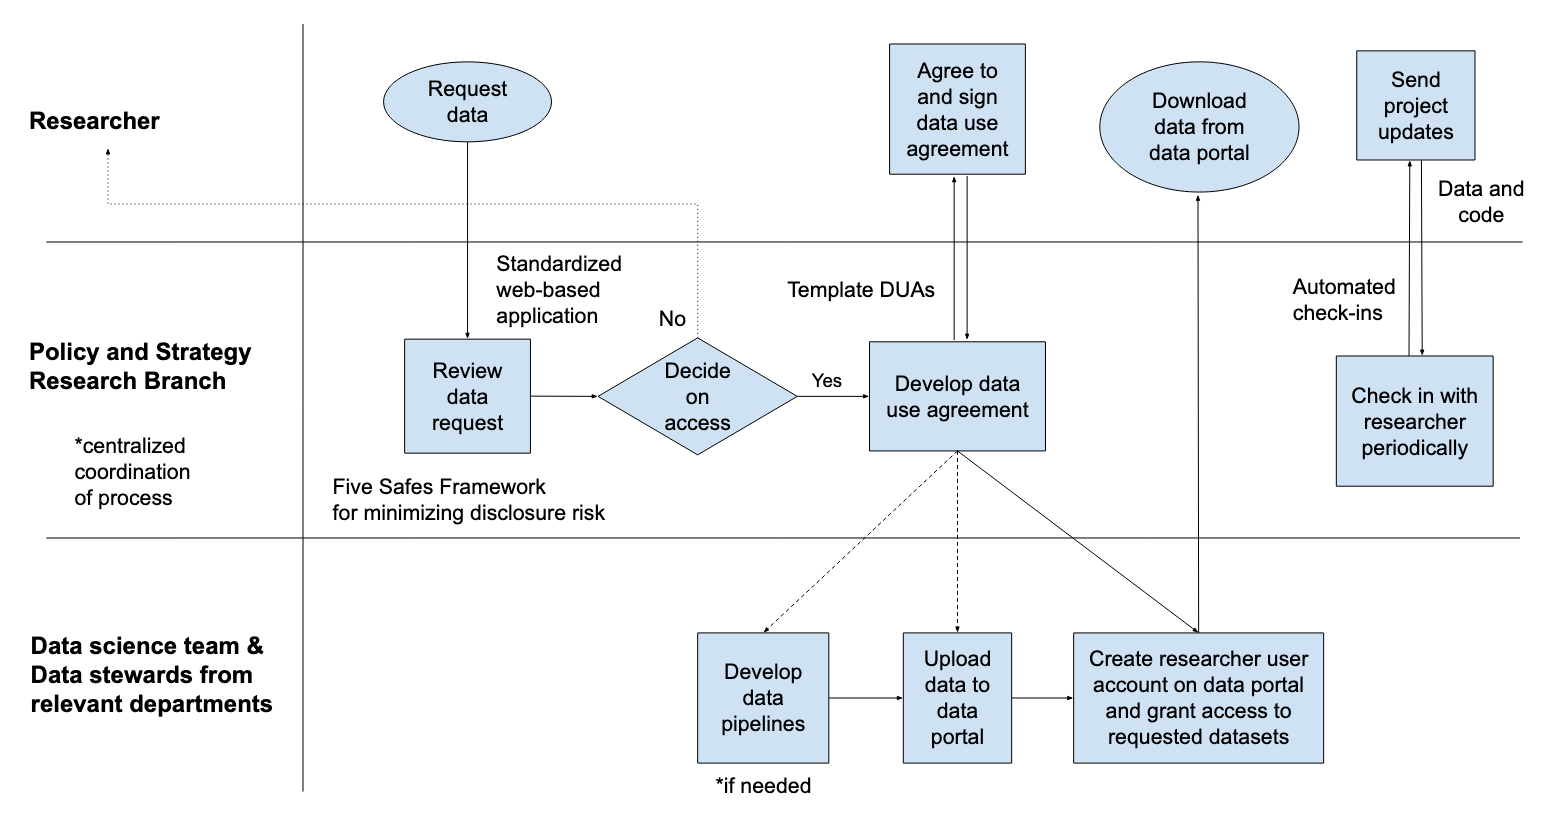
\includegraphics[width=1\linewidth]{./figures/cctfigure1} \caption{Data sharing process}\label{fig:cctfigure1}
\end{figure}

The process of identifying potential technical solutions for data streamlining has followed best practices by (1) perceiving and identifying various barriers to data access and use \citep{connelly2016, goerge2018, lane2008, petrila2018, abraham2019}, (2) assessing new tools and approaches for secure and remote access to data \citep{lane2008, culhane2018, foster2018}, and (3) understanding diverse user needs \citep{lane2018, abraham2019}.

Other important considerations and activities have revolved around the following areas listed in Table \ref{tab:ccttable1}. In all of these tasks and in implementation, investments in human capital with respect to data skills of CCT staff as well as network-building internally and externally are perceived as crucial to success.

% 
% \begin{table}
% %\footnotesize
% \caption{\label{tab:ccttable1}Areas of consideration and associated activities}
% \centering
% \begin{tabular}{p{10em}p{25em}}
% 	\toprule
% 	Task&Consideration\\
% 	\midrule
% 		\csvreader[late after line=\\]{./assets/cct/ccttable1.csv}{}%
% 		{\csvcoli & \csvcolii }%
% 	\bottomrule
% 	\end{tabular}
% 	%	
% \end{table}

\begin{table}

\caption{\label{tab:ccttable1}Areas of Consideration and Associated Activities}
\centering
\begin{tabulary}{1.0\textwidth}{lL}
\toprule
Technical solutions & - Finding a data sharing platform with sufficient metadata and access control capabilities to support researcher-specific use restrictions\\
                    & - Integrating said platform with CCT data systems\\
Data infrastructure & - Development of metadata standards\\
                    & - Assessment of self-hosting options versus cloud computing with the appropriate attention given to security concerns.\\
IT architecture 	& - Addressing tensions between existing and newer approaches and technology stacks\\
                    & - Ensuring that legacy systems do not create barriers to effective data sharing\\
Governance 	        & - Process improvement evaluations\\
                    & - Processes for integrating data use agreements with the data sharing platform\\
Data privacy        & The evolution of CCT's understanding and application of applicable data laws and data ethics considerations must keep pace with CCT's increasingly open data environment\\
\bottomrule
\end{tabulary}
\end{table}

\hypertarget{metadata-2}{%
\subsection{Metadata}\label{metadata-2}}

A major initiative to facilitate data use is the development and implementation of structured metadata standards\index{metadata standards} to be applied to all CCT data. CCT's Data Science team together with the Information and Knowledge Management department have developed standards comprising a minimal required set of \href{http://osf.io/2a7ev}{metadata elements} along with additional, recommended elements. The minimal set of elements is similar to the Dublin Core\index{Dublin Core} but with unique considerations for administrative data. The intent of the required minimal set is to minimize the burden on data stewards and to maintain quality metadata. Core fields include a summary of the data set, update frequency, data access rights, reasons for restriction, data format, spatial coverage, temporal coverage, and information about the source and stewardship of the data set.

CCT is investigating the process for making a publicly available catalog of all available CCT data that also contains basic metadata. This catalog could include both public-use and restricted-use data sets with the former providing direct access links and the latter providing information on how to request access to the data. An initial internal data inventory has been created, cataloging over 1,000 distinct data resources. Over 500 unique data resources come out of the SAP system used for revenue management and other administrative purposes. The GIS data system (run on ESRI software) is the second biggest source with nearly 500 unique data resources. Metadata creation and further classification are needed before it can be made public. Once completed, this data catalog will make it easier for researchers both inside and outside of CCT to identify specific data of interest and to include them in research requests: this will reduce the burden on CCT staff when processing requests. Additionally, the tacit knowledge gained by researchers through the experience of working with a particular data set can be codified by contributing back metadata and longer-form documentation. In particular, researchers' assessment of the quality and usability of the data is especially important \citep{connelly2016}.

\hypertarget{data-processing}{%
\subsection{Data Processing}\label{data-processing}}

CCT data are generated, in most cases, in the course of administering day-to-day municipal functions. Data typically need to be transformed to be useful for researchers. Historically, as described in the first data use example, raw data were extracted from various source systems and shared with researchers who then invested in cleaning and organizing the data for their research purposes. For example, residential billing data come from the files used to print household bills. These are text files with variables stored in strings and multiple languages (Afrikaans, English, and Xhosa). A large amount of code is needed to convert these files into formats appropriate for analysis. Researchers face a trade-off between cleaning all the available data, which would allow for future analyses, and only developing the specific data set they need for their immediate research goals.

Going forward, CCT's intent is to develop data pipelines that transform raw data into more readily usable forms. The process involves collaboration between CCT's Data Science unit and the specific CCT departments where data originates. Where relevant, it will also involve researchers who have invested previously in processing specific data sets. CCT is actively promoting the potential multi-use of data in the design of major data gathering efforts undertaken by the municipality. For example, the municipal building and land use application system is currently being reviewed and restructured to accommodate data access and analysis by multiple CCT departments as well as external research partners. For many of CCT's large data sets, however, significant data engineering work is needed, and it is often difficult to establish consistent identifiers across data sources depending on the relevant unit of observation. Challenges also arise in communication across software platforms, such as the SAP billing platform, the ESRI spatial data platform, and the point-of-sale prepaid electricity vending server. Transitioning more of CCT's administrative systems toward open-source software would help address some of these issues, but long relationships with proprietary platforms such as SAP and ESRI make that difficult. Discussions surrounding the feasibility of these transitions are underway.

CCT strives for a balance between maintaining good data practices throughout the organization through the establishment of standards and rules as well as ensuring that there is not an unsustainable burden falling on those tasked with data generation and maintenance. The greater the number of actors anticipated to use the data, the more effort is required to collect, structure, and maintain the data. Relying on office and field staff to generate and prepare data to a specific standard while maintaining the status quo with their current job assignments may easily overburden them: in turn this could jeopardize overall data quality and create resistance to increased data sharing. Current plans anticipate investing in data processing in response to data use requests, but in a manner that anticipates multiple uses of the data; once data are extracted and processed, the same steps do not need to be repeated for future requests. Minimal processing to preserve flexibility across future users involves transforming data into tabular formats with standardized variable names as well as other modifications like storing dates and times in ISO 8601 format.

The primary barriers to developing data pipelines include (i) lack of access internally within CCT, (ii) lack of basic data documentation and (iii) time constraints of staff with the necessary skills. The goal is to expand the use of APIs (Application Programming Interface) within CCT to address (i) and increased metadata creation to address (ii). Both should help address (iii).

\hypertarget{legal-and-institutional-framework-5}{%
\section{Legal and Institutional Framework}\label{legal-and-institutional-framework-5}}

\hypertarget{institutional-setup-5}{%
\subsection{Institutional Setup}\label{institutional-setup-5}}

CCT is both the custodian and provider of administrative data. External researchers submit requests for data that also outline their research aims, and the Research Branch within the Policy and Strategy Department reviews the application. The Research Branch filters requests based on their research priorities and other criteria established in the Research Framework and liaises with relevant departments within the City to assess the availability of data and appropriateness of the request. The volume of requests is considerable: in FY20, CCT received 136 research applications.

CCT has established an inter-departmental Data Coordinating Committee\index{Data Coordinating Committee} (DCC) led by the chief data officer. Each department has a representative on the DCC, nominated by the executive director. The rest of the committee is composed of workstream leads, key directors/managers who are responsible for resources key to the strategy, and technical specialists. This committee provides governance, structure, and oversight of CCT's data, specifically with regards to the following three areas:

\begin{itemize}
\tightlist
\item
  Improved governance---to facilitate the development of a CCT data strategy and the establishment of clear accountability, roles, and responsibilities for the management of information
\item
  Technology---to ensure the development of Information Technology platforms and tools to support and enable the management and integration of CCT data and information (also addressing issues of usability)
\item
  Content---to set in place policies, guidelines, and standard operating procedures (SOPs) for the management of CCT data and information content \citep{cityofcapetown2018}
\end{itemize}

The mandate of the DCC includes the following:

\begin{itemize}
\tightlist
\item
  Identifying data gaps and priorities
\item
  Working toward one source of custodianship of data
\item
  Managing the potential duplication of data and reporting
\item
  Ensuring the availability of data
\end{itemize}

The Data Strategy sets forth many desired outcomes including (i) data sets available in a usable format; (ii) an IT architecture that accommodates diverse data types (volume, variety, velocity); (iii) SOPs for good data practices; (iv) skilled personnel able to adapt to changing data and software environments; and (v) a widespread recognition of the value of data throughout CCT.

To achieve these outcomes five key, interlinked workstreams were established: data culture, data capabilities, data collaboration and partnerships, data architecture, and data governance \citep{cityofcapetown2018}. A workstream on economic analysis was added in 2019 to reflect the emphasis in the data strategy of improving the use of a wider range of economic analysis tools in CCT decision making. The Data Science unit focuses primarily on the technical and architectural components of the Data Strategy.

\hypertarget{legal-context-for-data-use-5}{%
\subsection{Legal Context for Data Use}\label{legal-context-for-data-use-5}}

The primary data privacy law in South Africa is the Protection of Personal Information Act\index{Protection of Personal Information Act} (POPI) of 2013 \citep{republicofsouthafrica2013}. Though the law is technically in effect, it has yet to be implemented and enforced: this has introduced uncertainty around how to comply with the law. It is expected to be implemented sometime in 2020 and includes a one-year grace period such that strict enforcement would begin in 2021 \citep{giles2020}. Because there is no precedent, there is little guidance on what practical measures to take in order to comply, though the law is similar to the European Union's General Data Protection Regulation\index{General Data Protection Regulation} (GDPR).

POPI has two primary clauses that affect the use of data containing personally identifiable information\index{personally identifiable information} by researchers. First, it states that sufficiently de-identified data leads to compliance with the law. This is also often required by university human subjects research review boards in situations where consent is difficult to obtain, such as with administrative records. The law is somewhat ambiguous as to what sufficiently de-identified data means as well as with the point at which de-identification must occur. Second, POPI states that legitimate research use of personally identifiable data is exempt from the law.\footnote{For example, Condition 4, section 15 (3) on the further processing of personal information states: ``The further processing of personal information is not incompatible with the purpose of collection if--- \ldots{} \emph{(e)} the information is used for historical, statistical or research purposes and the responsible party ensures that the further processing is carried out solely for such purposes and will not be published in an identifiable form.''} The precise interpretation of the limitations imposed by POPI for research purposes is still under discussion by lawyers in Cape Town and elsewhere. In practice, CCT intends to de-identify all shared data unless access to personal identifiers is essential to the proposed research and is governed by a data use agreement that ensures confidentiality and restricts further dissemination.

To comply with POPI, CCT currently uses a combination of de-identification techniques and a disclosure control framework that filters and prioritizes legitimate research requests (described in the next section). Looking ahead, CCT data custodians will flag data sets with personally identifiable information through a tag in the metadata, applied to either the entire data set or specific variables within it. Additionally, data custodians may also categorize the sensitivity of the data set based on criteria still under development. This metadata will provide a streamlined and systematic approach to managing confidentiality concerns and POPI compliance.

While standards for managing most administrative records are still evolving, standards around spatial data are more entrenched. The Spatial Data Infrastructure Act of 2003 delineates the ways that spatial data and metadata are collected, maintained, and published by public bodies in South Africa, primarily to ease integration of various data sources and to minimize costs \citep{republicofsouthafrica2003}. CCT complies with these standards and regulations when sharing spatial data of any kind. Given that property identifiers are often used for linking across different administrative data sets, spatial data linked to these identifiers are particularly sensitive in the case of CCT.

\hypertarget{legal-framework-for-granting-data-access-5}{%
\subsection{Legal Framework for Granting Data Access}\label{legal-framework-for-granting-data-access-5}}

At the time of writing, CCT employs DUAs\index{DUAs} to stipulate what data sets can be accessed by external users and how the data can be used, as well as to convey related management issues including non-disclosure. Typically, the DUAs are developed with input from CCT's Research Branch and Legal Services Department, as well as the specific operational departments that generate the data. The focus of the DUAs is ensuring data confidentiality. In the absence of legal repercussions for violation of the agreement, their efficacy depends on trust between the parties, as well as reputational considerations and a desire for future collaboration \citep{sexton2017}.

The negotiation and establishment of bespoke legal agreements to underpin data and research partnerships was found to be a considerable disincentive for CCT and its partners to collaborate, and uneven and inconsistent terms created risks to both parties. CCT's legal department has prioritized the development of a series of template collaboration agreements to be available to all departments as an \emph{off-the-shelf} governance tool to use in establishing data and research partnerships. Data sharing can work in both directions: in most cases, CCT provides the partner with access to administrative data and the partner shares output and analytical code or improved data sets at the end of the project. In some cases, however, CCT explicitly looks to partnerships to fill data gaps. The following types of research and data partners are accommodated within this series of template agreements.

\begin{itemize}
\tightlist
\item
  \emph{Research partners} include academic institutions or individuals seeking to conduct research utilizing administrative data. Template agreements will cover both embedded research or active collaborations and more hands-off data access for desk-based analysis.
\item
  \emph{Knowledge partners} are organizations (private or public) who have data expertise and want to partner with CCT on specific projects.
\item
  \emph{Data partners} include government departments, businesses, and organizations who have data that the CCT requires to gain the insights necessary for better decision making. These agreements involve data sharing in the opposite direction (CCT is the recipient).
\item
  \emph{Donors} are funders who wish to support initiatives around data access.
\item
  \emph{Public sector partners} are public entities who can offer CCT technical support in implementing the City's Data Strategy, such as the National Treasury's CCT Support Programme and the UK Foreign Office-funded Future Cities Programme.
\item
  \emph{Contracted service providers} are contractors involved in implementing policies, programs, and day-to-day operations. Data sharing goes in both directions with contractors accessing CCT records and sharing data sets resulting from their activities back with CCT.
\end{itemize}

\href{https://resource.capetown.gov.za/documentcentre/Documents/Bylaws\%20and\%20policies/Intellectual_Property_Policy.pdf}{CCT's Intellectual Property Policy} provides guidance on Intellectual Property (IP) from publicly funded research and development, which is subject to case-by-case review. For non-commercial research output, CCT does not typically exert any IP ownership. IP of the original and derived data (not including statistical outputs) is retained by CCT, and acknowledgement of data sources is required in any resulting publications or public materials.

\hypertarget{protection-of-sensitive-and-personal-data-the-five-safes-framework-5}{%
\section{Protection of Sensitive and Personal Data: The Five Safes Framework}\label{protection-of-sensitive-and-personal-data-the-five-safes-framework-5}}

CCT balances the need to extract value from data with the need to protect the privacy and interests of residents, as well as the security of CCT's physical assets. New approaches in data sharing must be accompanied by stringent security measures and robust data governance for the municipality to fulfil its responsibility to respect and protect its residents.

As part of the Data Strategy, CCT is pursuing a secure distribution model for sharing data, primarily as downloads via a secure, access controlled, cloud-based data sharing platform\index{data sharing platform}, which allows more flexibility than a data enclave\index{data enclave} model but carries a greater disclosure risk. While CCT has had existing disclosure control practices, they have not been motivated by an explicit framework or conceptual model. Currently, CCT is re-evaluating its practices as guided by the Five Safes framework \citep{desai2016}. In contrast to a data enclave model, secure distribution arguably relies more heavily on project selection and data use agreements to minimize disclosure risk, relative to technical means that place strong limits on where data can be stored and analyzed. The choice of secure distribution results from concerns over the costs of implementing a data enclave model, and restrictions on access if implemented as a physical enclave. In addition, risks are mitigated by the relatively low assessed risk of most CCT data that is shared for research purposes.

A data sharing platform\index{data sharing platform}---defined here as a centralized, cloud-based location for securely cataloging, describing, uploading, controlling access to, and downloading data sets---facilitates numerous aspects of the proposed streamlining. In order to achieve a streamlined process, the platform should integrate both the technical aspects of securely storing and distributing data with the governance aspects of controlling access to data. Additionally, as a data catalog at the core, the platform should serve as a data discovery tool based on the available metadata for both internal and external research purposes. Currently, CCT is working toward adopting a modified version of CKAN, which is a popular open-source data sharing platform. CKAN is primarily designed and used for sharing open data sets, so modifications are needed to extend its access control and security capabilities.

The authors assess each of the Five Safes in light of CCT's reworking of the data sharing framework (1 = least important, 5 = most important).

\hypertarget{safe-projects-5}{%
\subsection{Safe Projects}\label{safe-projects-5}}

Importance = 5; Cost = 5

In the future, project selection will be based on a formal application that specifies research questions and required data, though historically this has not always occurred. The Research Branch reviews the applications for appropriateness and alignment with the \href{http://osf.io/2a7ev}{Research Framework and research priorities} (see section Institutional setup above). Currently, the review workflow has associated SOPs, though areas of improvement have been identified, especially with respect to integration with the entire data sharing process. For example, the application process could trigger determination of security levels (linked to tags in the metadata) and eventual access restrictions. The application form is being redesigned as a web-based form to make it more accessible to external researchers and to help reduce processing time. Domain experts, analysts, and lawyers may all review applications, and applications are reviewed in the order that they are received. Where necessary, the research application triggers the development of a DUA, as described under the section Legal framework for granting data access (above). In the future, a rule may be added that institutional review board (IRB) approval is needed before access is formally granted to academic researchers: a requirement that benefits from publicly accessible metadata.

\hypertarget{safe-people-5}{%
\subsection{Safe People}\label{safe-people-5}}

Importance = 5; Cost = 3

CCT accepts applications from what it views as trusted researchers with institutional affiliations. Many of the filters applied to identify trusted researchers are anticipated by the template agreements described under the section Legal framework for granting data access (above). Under current practices, the specific cost of verifying trusted researchers is lower than the overall assessment of a proposed project. Because CCT will use a secure distribution model, it places additional importance on selecting safe people. However, there are no specific requirements or training needed apart from having a relevant qualification, demonstrable research experience, and an institutional affiliation: all of which signal a basic competency in data management and analysis. Drawbacks of this approach include (a) that some early career or less well-established researchers may be overlooked and (b) guidelines for implementation remain subjective.

\hypertarget{safe-settings-5}{%
\subsection{Safe Settings}\label{safe-settings-5}}

Importance = 4; Cost = 3

If a research application is accepted, a DUA\index{data use agreement} is then developed. The primary purpose of this agreement is to ensure the nondisclosure of confidential information by describing the specific data that can be used and how it can be stored and analyzed. It is intended that data will be distributed primarily through secure downloads, but other means like encrypted flash drives may also be used in certain cases. This improves flexibility in the location of the actual research. The agreements make it clear, however, that the responsibility for properly and securely managing data falls on the researcher who is liable for any breaches or disclosures. The selection of trusted researchers helps minimize the risk in this area, though additional requirements such as (third-party) training in safely accessing and storing confidential data would further reduce risks.

\hypertarget{safe-data-5}{%
\subsection{Safe Data}\label{safe-data-5}}

Importance = 4; Cost = 2

Safe data is ensured by initially assessing the risk of requested data for individual data sets and their combination. Additionally, data containing personally identifiable information\index{personally identifiable information} are de-identified when possible, and aggregated data may also be made available instead (when appropriate to the research design). The data use agreement also stipulates that the data must be used exclusively for research purposes and may not be used for economic or other advantage or distributed to others. Once again, the selection of trusted researchers helps minimize the risk in this area.

Making data safe is less costly than the existing procedure of extracting and processing data for each individual request, which often involves repeating extractions that other researchers have requested in the past. To populate the secure data platform following an approved research request, raw or minimally processed data will be extracted, organized, and shared on the platform with complete metadata to ensure users are familiar with the data generating process and interpretation of the data content. CCT is currently working to develop data pipelines that will help reduce the internal burden of processing and de-identifying data and not require re-extractions of the same data. The sensitivity of a data set will be ranked and tagged in metadata to enable quicker risk assessments, and less sensitive versions of data sets may be generated by, for example, aggregating or averaging across observations. However, currently there are no plans to use additional methods such as sampling or adding noise to the data. Beyond these steps, the burden of transforming data into a research-ready format falls on the researcher, and it is intended to require researchers to share code and processed data through the data platform for use by CCT.

\hypertarget{safe-outputs-5}{%
\subsection{Safe Outputs}\label{safe-outputs-5}}

Importance = 2; Cost = 1

Safe outputs are ensured by a review of papers and other research outputs by CCT staff, though the onus primarily falls on the researcher. DUAs\index{DUAs} typically state that the researcher should provide a manuscript to CCT prior to publication and CCT then has 30 days to review and respond with respect to disclosure issues. Researchers do not always comply because research relationships are often one-off, deadlines are not clearly defined, and CCT is left to chase after researchers who fail to supply a manuscript. Specific deadlines could be added via the researcher's login to the data sharing platform, and access could be limited if research output is not shared on time. Going forward, CCT intends to catalog all research that is produced from CCT data. The data sharing platform can be leveraged to streamline this process.

\hypertarget{data-life-cycle-and-reproducibility-1}{%
\section{Data Life Cycle and Reproducibility}\label{data-life-cycle-and-reproducibility-1}}

\hypertarget{preservation-and-reproducibility-of-researcher-accessible-files-4}{%
\subsection{Preservation and Reproducibility of Researcher-Accessible Files}\label{preservation-and-reproducibility-of-researcher-accessible-files-4}}

As mentioned previously, the data sharing process will eventually be embedded in broader research management practices by CCT. To some extent, such as with the metadata standards, data, and code curation practices are also under development. Because of the costs in terms of personnel time and resources, these practices are currently limited. The proposed data sharing platform will maintain access to data indefinitely, but more thought needs to be given to long-term preservation in terms of storage, persistent identifiers, version control, and access permissions. This is an area where partnership with research organizations could be fruitful.

\hypertarget{preservation-and-reproducibility-of-researcher-generated-files-3}{%
\subsection{Preservation and Reproducibility of Researcher-Generated Files}\label{preservation-and-reproducibility-of-researcher-generated-files-3}}

The reciprocal sharing of researcher-generated files back to CCT is desired and intended to be explicitly embedded in DUAs\index{DUAs}, but it remains to be seen how to share materials effectively. CCT places greater emphasis on code sharing because code documents the analysis workflow and derived data files can always be re-generated, though this depends on how robustly CCT preserves source data sets. In addition, code typically does not need to be access controlled and could be publicly shared, ideally via Git repositories. By detailing the workflow, this would increase research transparency, reproducibility, and productivity \citep{playford2016}. Integrating exchange of code via the data sharing platform is also under consideration.

\hypertarget{sustainability-and-continued-success-5}{%
\section{Sustainability and Continued Success}\label{sustainability-and-continued-success-5}}

\hypertarget{outreach-4}{%
\subsection{Outreach}\label{outreach-4}}

The Policy and Strategy Department, especially its Research Branch, implements the research management functions for CCT for both internal and external activities. These functions include reviewing data requests and project proposals and developing data use agreements.

In addition, the data platform being developed provides an access point to CCT's data both in terms of metadata as well as secure downloads. A web-based data request form is also in development.

Apart from managerial functions, the Policy and Strategy department and its Research Branch also facilitate and coordinate institutional research partnerships and knowledge networks. These networks include a diverse set of researchers and organizations covering multiple disciplines, geographies, levels of experience, and research interests. CCT collaborates with the \href{http://www.chec.ac.za}{Cape Higher Education Consortium} and has other long-standing research partnerships (e.g., with \href{https://www.mistraurbanfutures.org}{Mistra Urban Futures} and the \href{https://www.africancentreforcities.net}{African Centre for Cities}). CCT is building on this foundation by actively seeking new research partnerships locally and internationally; the City is seeking to establish formal collaborations with universities where there is already evidence of research partnering with multiple researchers at an institution.

\hypertarget{revenue-4}{%
\subsection{Revenue}\label{revenue-4}}

CCT chooses not to charge access fees to researchers, primarily because doing so would only serve to restrict access. Though CCT incurs costs to share data with researchers, it expects value returned in the form of useful knowledge and related products, such as cleaned data sets and analysis code. Supporting research (and students) is also treated as creating a public good. Charging fees would likely disadvantage many researchers in South Africa and other developing countries.

CCT's rationale for investing in a more streamlined process for data sharing and collaboration is premised on cost-saving rather than revenue generation. A lack of internal capacity for data science, statistics, and economic analysis means that CCT needs to harness partnerships with external researchers to realize the value of its data. One of the five pillars of the Data Strategy is the fostering of research partnerships to mitigate the risk of overburdening CCT staff or overutilizing expensive consultant time. Additionally, CCT recognizes that it can never recruit and retain all the knowledge and specialized skills it needs to understand and respond to complex urban challenges. Where incentives can align, research partnerships give access to this expertise and insight.

\hypertarget{metrics-of-success-4}{%
\subsection{Metrics of Success}\label{metrics-of-success-4}}

CCT's Research Framework outlines monitoring and evaluation indicators for both internal and external research projects, although operationalizing the indicators is a work in progress. Metrics include the number of research analyses that directly inform CCT strategy, policy and by-law processes and operations, the number of CCT programs influenced by research analyses, and the number of CCT-supported research engagements. In addition, metrics will cover the number of specialist research studies initiated by CCT staff (experimental, modelling, evaluation, feasibility, longitudinal, predictive) and the number of CCT research platforms and tools accessed, among others.

In lieu of revenue generated by selling data, CCT intends to track the monetary value of research funding raised through its partnerships (even if the funds stay with the researchers) and the estimated value of the services provided by researchers. These values will be calculated by pricing the estimated hours of external researcher time according to the standard consultancy rate for the level of skills and tasks completed. In addition, CCT will estimate the monetary value of external expertise gained in the form of time and tools, techniques, models, and systems developed. These metrics will be useful in building the business case for investment in external partnerships by CCT.

More directly related to data sharing between CCT and researchers, metrics will track the number of data sets made available to strategic partners (with necessary agreements in place) and the time required for external partners to gain access to CCT data; where possible, metrics will be tracked according to sensitivity rankings (open, sensitive, confidential).

\hypertarget{concluding-remarks-2}{%
\section{Concluding Remarks}\label{concluding-remarks-2}}

This case study provides a snapshot---taken in the midst of a dramatic transformation in Cape Town---where the municipality is purposefully implementing a Data Strategy and Research Framework and creating a unique and secure data sharing platform. Importantly, this platform will meet the needs of internal users, lowering the cost of in-house data discovery and exchange. At the same time, these internal efforts are being leveraged to streamline data sharing with external researchers whose research proposals have been vetted by CCT staff. Using the platform, researchers will be able to search for available data, securely download data to which they have been granted access, and contribute metadata, analysis code, and other files.

The benefits of streamlining the data sharing process include an increased volume of research on policy relevant questions, greater accountability of researchers to report findings and share cleaned data or new data sets with CCT, and a more secure and standardized approach to transferring data to researchers. These benefits come at a cost, which is largely front-loaded and associated with establishing the data sharing platform, as well as centralizing and standardizing the diverse set of administrative data sets used by CCT. This stage is still ongoing, and the interim picture provided here is rapidly changing. Lessons will continue to be learned and unresolved issues solved. CCT will carefully balance data privacy concerns with the need to generate bodies of evidence that inform municipal policies and support enhanced service delivery and improved outcomes for residents of Cape Town.

\hypertarget{supplemental-materials}{%
\section*{Supplemental Materials}\label{supplemental-materials}}
\addcontentsline{toc}{section}{Supplemental Materials}

The video of this chapter's webinar presentation can be found here (link to come). The slides for the webinar presentation are available here (link to come).

\hypertarget{about-the-authors-7}{%
\section*{About the Authors}\label{about-the-authors-7}}
\addcontentsline{toc}{section}{About the Authors}

Hugh Cole has been director of Policy and Strategy at the City of Cape Town since 2017. The Policy and Strategy Department contains four branches: Strategic Policy, Strategic Planning, Research, and Economic Analysis. He reports to the executive director of Corporate Services (also the Chief Data Officer). Prior to joining CCT, Hugh was the Director responsible for Country Programmes at the \href{http://www.theigc.org}{International Growth Centre} (IGC) based at the London School of Economics (LSE). Hugh is a graduate of the University of Cape Town and the LSE where he is Visiting Fellow of the School of Public Policy.

\href{http://kelseyjack.bren.ucsb.edu/}{Kelsey Jack} is an Associate Professor of Environmental and Development Economics at the University of California Santa Barbara's Bren School of Environmental Science and Management. She has conducted research, including RCTs and observational studies, in collaboration with CCT since 2013. She co-chairs J-PAL's Environment, Energy, and Climate Change sector and is on the advisory board for J-PAL Africa's IDEA Lab. She is also lead academic for IGC Zambia and a Faculty Director of UCSB's Environmental Market Solutions Lab (emLab).

\href{https://drkrynstrng.gitlab.io/}{Derek Strong} is currently a Research Computing Associate with the Center for Advanced Research Computing at the University of Southern California. Prior to this, he worked with Kelsey Jack at UC Santa Barbara and with the City of Cape Town to identify and implement solutions for streamlining municipal data sharing with researchers. His interests include research computing, open science, and meta-research.

\href{https://sites.google.com/site/bmaughanbrown/}{Brendan Maughan-Brown} is an interdisciplinary social scientist with expertise on: the uptake of HIV-prevention and treatment services; behavioural economics; and the social and behavioural determinants of HIV risk. He is a Chief Research Officer at the Southern Africa Labour and Development Research Unit, University of Cape Town.

\hypertarget{acknowledgements-3}{%
\section*{Acknowledgements}\label{acknowledgements-3}}
\addcontentsline{toc}{section}{Acknowledgements}

The authors thank Gordon Inggs, Yogini Jivanji, Craig Kesson, Kayleen Simpson, Carol Wright, Joshua Hawley, and the IDEA team at J-PAL for support of the collaboration and for constructive comments on the draft.

\putbib

\FloatBarrier\newpage

\hypertarget{appendix-6}{%
\section*{Appendix}\label{appendix-6}}
\addcontentsline{toc}{section}{Appendix}

\hypertarget{appendix-a-2}{%
\subsection*{Appendix A}\label{appendix-a-2}}
\addcontentsline{toc}{subsection}{Appendix A}

\hypertarget{summary-of-data-strategy-implementation-june-2020}{%
\subsubsection*{Summary of Data Strategy Implementation (June 2020)}\label{summary-of-data-strategy-implementation-june-2020}}
\addcontentsline{toc}{subsubsection}{Summary of Data Strategy Implementation (June 2020)}

Below are the guidelines used to conduct implementation of the Data Strategy, as of June 2020. This summary describes the Data Strategy Implementation document which is not publicly available.

\hypertarget{data-governance}{%
\subsubsection*{Data Governance}\label{data-governance}}
\addcontentsline{toc}{subsubsection}{Data Governance}

\begin{itemize}
\tightlist
\item
  Making data searchable and managing data quality improves its usability for evidence-informed decision making.
\item
  CCT undertook exercises to understand all data sets and metadata held by the City.
\item
  CCT is developing a data taxonomy of the hierarchical relationships between data sets.
\item
  CCT is developing a data dictionary of terminology and metrics. The data dictionary will standardize usage across units within CCT and improve efficiency in communication and collaboration on data projects.
\item
  An institutionalized data governance structure ensures quality data. Empowering data collectors and generators to take ownership of the data and its quality can improve data cleaning. Human efforts can be augmented by advanced analytics that can detect anomalies and surface uncleaned data.
\item
  CCT also provides standards for data analytics to ensure that the results provided by data analysts can be reproduced and verified.
\item
  CCT uses open-source software, where possible, to scale analytical efforts in collaboration with service providers and academics, to reduce the time constraints of the procurement process, and to reduce the time from design to institutionalization, implementation, and outcome.
\end{itemize}

\hypertarget{data-culture}{%
\subsubsection*{Data Culture}\label{data-culture}}
\addcontentsline{toc}{subsubsection}{Data Culture}

\begin{itemize}
\tightlist
\item
  CCT's initiatives build institutional knowledge to flexibly manage data and adjust to changes both internally and externally.
\item
  A change management plan is being rolled out to create awareness of, and desire for, working with data.
\end{itemize}

\hypertarget{data-capabilities}{%
\subsubsection*{Data Capabilities}\label{data-capabilities}}
\addcontentsline{toc}{subsubsection}{Data Capabilities}

\begin{itemize}
\tightlist
\item
  CCT invests in human resources to develop and manage open data architectures.
\item
  Roll-out of training programs will build capacity with data analysts, data scientists, data engineers, data governance experts, data stewards, data custodians, user interface designers, web developers, data collectors, and other staff.
\item
  Introducing a data literacy program will educate the organization as a whole on understanding and communicating with data.
\item
  Data engineering efforts will build the necessary data infrastructure that will bring CCT into the big-data world, with a strong technical foundation for future analysis for decision-making.
\item
  Guidelines on appropriate methods for data gathering and acquisition will be established.
\item
  Strategizing survey efforts will maximize value from data collection, for example by combining household and health surveys into a single exercise.
\item
  Open-source software can increase transparency and decrease the barrier to entry for new staff who often face a steep learning curve to understand proprietary and customized software.
\item
  Sandbox data science and analytics environments are provided to staff, allowing allows them to fail, experiment, and learn.
\item
  The City of Cape Town has expertise in urban monitoring and policy, but lacks the data engineering capacity to transform a data source into a useful tool for managers and policy makers. The City needs to build capacity within existing staff and employ data professionals to augment internal skills and increase data utilization. Cape Town's proximity to three major universities---the University of Cape Town, Stellenbosch University, and the University of the Western Cape---brings hundreds of skilled professionals to CCT.
\end{itemize}

\hypertarget{appendix-b-1}{%
\subsection*{Appendix B}\label{appendix-b-1}}
\addcontentsline{toc}{subsection}{Appendix B}

\hypertarget{research-branch-project-review-criteria-based-on-research-framework-prioritization-june-2020}{%
\subsubsection*{Research Branch project review criteria based on Research Framework prioritization (June 2020)}\label{research-branch-project-review-criteria-based-on-research-framework-prioritization-june-2020}}
\addcontentsline{toc}{subsubsection}{Research Branch project review criteria based on Research Framework prioritization (June 2020)}

This outline of CCT's Research Branch project review criteria summarizes the document, which is not publicly available. The outline is a resource for CCT's strategy and priorities driving research to inform policy.

CCT research focus areas and questions will be prioritized according to certain criteria, including the following:

\hypertarget{research-that-is-linked-to-the-core-functions-of-ccts-constitutional-mandate}{%
\subsubsection*{Research that is linked to the core functions of CCT's Constitutional Mandate}\label{research-that-is-linked-to-the-core-functions-of-ccts-constitutional-mandate}}
\addcontentsline{toc}{subsubsection}{Research that is linked to the core functions of CCT's Constitutional Mandate}

\begin{itemize}
\tightlist
\item
  The foundation of the City's research focus is to inform the City's strategy and policy review cycle(s) and sectoral and departmental strategies and plans.
\item
  Local government has been entrusted with public funds and resources in order to fulfil a specific mandate, as envisioned by South Africa's democratic founders and documented in the Constitution. Research questions within this mandate are prioritized.
\item
  It is CCT's responsibility to use its public funds and resources as efficiently and effectively as possible in fulfilling this mandate. Hence, the research in which CCT invests must further this cause.
\item
  CCT's research interests must not be restricted only to what functions it currently undertakes, given that the context in which local government must fulfil its mandate is ever-changing. Research questions can shape CCT's social, economic, and environmental future, so research that is not directly tied to current policy decisions must also be prioritized.
\item
  Research plays an important role in ensuring CCT adapts to new trends and environments by informing future decisions and proposals for action.
\item
  Research topics likely to be of interest to external researchers will be considered. Preference will be given to high-quality doctoral and postdoctoral research.
\end{itemize}

\hypertarget{research-that-will-be-utilized-to-inform-current-and-future-decisions}{%
\subsubsection*{Research that will be utilized to inform current and future decisions}\label{research-that-will-be-utilized-to-inform-current-and-future-decisions}}
\addcontentsline{toc}{subsubsection}{Research that will be utilized to inform current and future decisions}

Policy decisions are a function of the decision-making environment and the potential for impact on the wellbeing of Cape Town residents.

\hypertarget{decision-making-environment}{%
\paragraph{Decision-making environment}\label{decision-making-environment}}
\addcontentsline{toc}{paragraph}{Decision-making environment}

\begin{itemize}
\tightlist
\item
  Research that will inform clear options for decision-makers, providing understanding of complex issues and predicting potential impact of policy decisions, will be prioritized.
\item
  Research will be a decision-making tool when policy options are unclear and both intended and unintended consequences difficult to predict.
\item
  Research can assist to identify and monitor new trends and possible risks.
\item
  Research on key themes can increase CCT's understanding of underlying dynamics on a local issue.
\item
  CCT will prioritize cutting-edge research on high-value topics of interest.
\end{itemize}

\hypertarget{the-potential-impact-of-the-decision}{%
\paragraph{The potential impact of the decision}\label{the-potential-impact-of-the-decision}}
\addcontentsline{toc}{paragraph}{The potential impact of the decision}

\begin{itemize}
\tightlist
\item
  Research linked to decisions with a greater potential impact will be prioritized.
\item
  Impact can be understood as a function of the following elements:

  \begin{enumerate}
  \def\labelenumi{\alph{enumi}.}
  \tightlist
  \item
    Budget/Resource implications in both the short- and long-term taking note of the following:

    \begin{itemize}
    \tightlist
    \item
      Technical debt: Some policies may have lower capital outlays initially but may require technology or a technical approach that will incur significant maintenance costs over time.
    \item
      Opportunity cost: When resources are allocated to implement a policy, what other policies are not implemented? What are the potential benefits for CCT residents of the chosen policy and of the policies that are not chosen?
    \end{itemize}
  \item
    Risk

    \begin{itemize}
    \tightlist
    \item
      The extent of known risks associated with a decision and the impact of these risks on the wellbeing of the residents of Cape Town, as well as on the natural environment.
    \item
      The potential for unknown risks associated with a decision, whereby unintended consequences stemming from a decision could yield negative impacts.
    \end{itemize}
  \item
    Finality

    \begin{itemize}
    \tightlist
    \item
      The extent to which a decision can be adjusted over time in accordance with feedback received on its impact.
    \item
      Policies and decisions that require high capital investment can be difficult to adjust or course-correct. In such cases, generating information and informing decisions with evidence is key.
    \end{itemize}
  \end{enumerate}
\end{itemize}

\hypertarget{research-to-evaluate-the-impact-of-past-decisions}{%
\subsubsection*{Research to evaluate the impact of past decisions}\label{research-to-evaluate-the-impact-of-past-decisions}}
\addcontentsline{toc}{subsubsection}{Research to evaluate the impact of past decisions}

\begin{itemize}
\tightlist
\item
  Research that evaluates the impact of a policy decision over time is prioritized according to the budget and resource implications of a policy as well as its associated risks.
\item
  Program and project evaluation are often difficult, particularly when trying to ascertain impact as opposed to outcomes or outputs.
\item
  Funding and resources may be allocated for intensive impact assessments, beyond the scope of the routine Performance Management activities of CCT.
\end{itemize}

\hypertarget{research-that-supports-the-city-in-experimenting-with-policy-or-operational-responses-to-complex-problems}{%
\subsubsection*{Research that supports the City in experimenting with policy or operational responses to complex problems}\label{research-that-supports-the-city-in-experimenting-with-policy-or-operational-responses-to-complex-problems}}
\addcontentsline{toc}{subsubsection}{Research that supports the City in experimenting with policy or operational responses to complex problems}

\begin{itemize}
\tightlist
\item
  Research enables the City to be agile and innovative in response to increasingly complex problems, and to understand the challenging and rapidly changing context in which the City plans, manages, and operates.
\item
  The City will approve research that supports new policy or operational alternatives to assist the City in making decisions and informing actions, with the goal of responsive and effective service delivery.
\end{itemize}

\hypertarget{appendix-c}{%
\subsection*{Appendix C}\label{appendix-c}}
\addcontentsline{toc}{subsection}{Appendix C}

These are the metadata elements that are required by general data users in establishing what data exists, how it can be accessed, and potential uses of the data. These are the minimum requirements for adding a dataset to the municipal data catalog.

\begin{table}

\caption{\label{tab:cctapptabdata}Core Metadata Elements for Municipal Datasets (June 2020)}
\centering
\begin{tabulary}{1.0\textwidth}{lLL}
\toprule
Element Name & Description & Notes\\
\midrule
Unique ID & Unique ID for dataset & \\
Dataset Name & A name given to the dataset & Should be short but adequately reflect to what the content of the dataset relates\\
Dataset Description & A summary of the dataset, including contents and usage by CCT & Should include purpose/usage of the dataset and how the data is sourced/acquired\\
Dataset Quality & Subjective assessment of dataset quality & Should indicate specific gaps or concerns\\
Update Frequency & Frequency with which the data are updated in the dataset. Helps researcher understand how often the content is likely to be changed and whether it might be dependent upon a regular event, such as an annual budgetary process & Historical (not updated), Event Based\\
\addlinespace
Data Access Rights & Classification of the dataset in terms of access & Open Public, Internal Open, Internal Restricted, Secret\\
Restricted Reason & To be completed if the dataset is classified as Restricted; Indicates the reason for restricting access & Personal Information, Security\\
Data Format & Provides an indication of the interoperable structure of the data as reflected by the primary file format in which the system exports data & Examples include: CSV, Relational DB, Excel, Word, PDF, Text, MP4, MPEG\\
Data Steward & Indicates the individual who assumes business accountability for the dataset in relation to aspects such as access, quality, integrity, and completeness & Should be a person who has sufficient authority to authorize decisions in relation to the management of, and access to, the dataset; if the dataset is sourced from an external organization, the data steward should be from the department primarily responsible for obtaining the data on behalf of CCT\\
DS/TR Branch & Indicates the organizational unit (branch) of the data steward & \\
\addlinespace
DS/TR Department & Indicates the organizational unit (department) of the data steward & \\
DS/TR Directorate & Indicates the organizational unit (directorate) of the data steward & \\
Data Contact & Indicates the official who works most closely with, and can best provide additional information about, the data and metadata & \\
Data Custodian & Indicates the official who is responsible for the technical management of the data (e.g., the hosting and serving of the data) & \\
Host System ID & Unique ID of the application in which the data are stored (primary/source system) & \\
\addlinespace
Spatial Coverage & Indicates areas for which data are recorded & Entire city or subareas; Should also indicate the lowest spatial unit at which the data can be presented/analyzed\\
Temporal Coverage & Indicates the range of time for which data are recorded & Specific dates or intervals when data were recorded; Earliest and latest dates for which data were recorded\\
\bottomrule
\end{tabulary}
\end{table}

